% !TEX root = ../main.tex
\chapter{Sentiment Analysis}
\label{ch:sentimentAnalysis}

Semantic orientation describes the strength and polarity of words and phrases used in text.
Extraction of subjectivity and polarity of the text from the semantic orientation of its words and phrases is called sentiment analysis.
The huge volume of text-based interactions on social media makes it difficult
to read and organize them, and manually analyze their sentiment.
Focusing on single instances of interaction also makes it difficult to extract the overall sentiment,
necessitating a solution that performs and summarizes the analysis automatically, fast, and gives human-comprehensible results~\cite{Sarlan2014}.

\section{Methods}
\label{sec:methods_sa}

The informal language used in statuses on Twitter, and the limited length, poses an additional difficulty
to analyzing their sentiment.
Previous research showed supervised approaches to be superior to lexicon-based approaches~\cite{Sarlan2014}.
Since labeled data is available from the Sanders dataset~\cref{sec:theSandersDataset},
this thesis will focus on supervised approaches.
The dataset was preprocessed using the preprocessing and tokenization functions introduced in~\cref{sec:preprocessingAndTokenization} (without stopwords removal),
and the following methods evaluated.

\subsection{Naive Bayes}
\label{subsec:naivebayes}

The naive Bayes algorithm works by first expressing the probability of a label given the features,
in this case the sentiment given the bag of words that is the status, with Bayes rule:

\begin{equation}
    P(label|features) = \frac{P(label)*P(features|label)}{P(features)}
\end{equation}

The algorithm then naively assumes that all features are independent, giving:

\begin{equation}
    P(label|features) = \frac{P(label)*P(feature 1|label)*...*P(feature n|label)}{P(features)}
\end{equation}


The denominator $P(features)$ is not explicitly calculated.
Instead, all numerators are calculated and the denominator is chosen such that all $P(label|features)$ sum to 1~\cite{nltkDocs}.
\\
The features of each status are extracted as a vector of every distinct word in the dataset,
together with $True$ if the word can be found in the status, or $False$ if not.
The Python-code achieving this encoding can be seen in~\cref{code:extract_features}.

\begin{figure}
    \caption{Encoding a status as a vector}
    \label{code:extract_features}
    % @formatter:off
    \begin{minted}{python}
        features = {} # Contains every word in the dictionary and whether the status contains it.
        # Using the previously created dictionary
        for word in dictionary:
            features['contains(\%s)' \% word] = (word in document_words)
    \end{minted}
    % @formatter:on
\end{figure}

NLTK's implementation of this algorithm is used~\cite{nltkDocs}.
This implementation assumes the distribution of each feature $P(feature_i|label)$ to be multinomial,
making it a multinomial naive Bayes, which has shown the best performance in previous work~\cite{Go2009}.
The data from the Sanders dataset created in~\cref{sec:theSandersDataset} was shuffled and split into 10\% test data and 90\% training data,
which still gives accurate test results without removing too much from the little available training data.
This classifier achieved an accuracy of 75\%.
In addition to accuracy, the performance measures precision, recall and F-measure, were computed for this classifier.
Let $p_t$ be the number of statuses from a class that were actually labeled as being in that class,
and $p_f$ be the number of statuses from other classes that were falsely labeled as being in that class.
Similarly, let $n_t$ be the number of statuses that were correctly labeled as $not$ being in that class,
and $n_f$ be the number of statuses were labeled as not being in that class although they are.
The definitions for precision, recall and F-measure are then defined as follows:

\begin{equation}
    Precision = \frac{p_t}{p_t + p_f}
\end{equation}
\begin{equation}
    Recall = \frac{p_t}{p_t + n_f}
\end{equation}
\begin{equation}
    F-Measure = \frac{2 \times Precision \times Recall}{Precision + Recall}
\end{equation}

Intuitively, precision and recall can be understood as the percentage of positives that are real positives,
and the percentage of real positives that were labeled as positives, respectively.
The F-measure is their harmonic mean.
These measures, for each sentiment-class, can be seen in~\cref{tab:mnb_results}.
Class distribution and absolute counts for each class can be seen in~\cref{tab:naive_bayes_results}.

\begin{table}
    \centering
    \fontsize{8.5}{9}\selectfont
    \caption{Sentiment classification results using multinomial naive Bayes}
    \label{fig:sentiment_results}
    \begin{subtable}{.48\textwidth}
        \caption{Absolute counts and percentages}
        \label{tab:naive_bayes_results}
        \centering
        \begin{tabular}{lllll} %
            \toprule
            & \multicolumn{2}{c}{Test Data} & \multicolumn{2}{c}{Classification Result}\\
            \cmidrule{2-3}
            \cmidrule{4-5}
            Sentiment
            & Count
            & Percentage
            & Count
            & Percentage
            \\\midrule
            neutral & 206 & 47\%  & 266 & 61\%
            \\\midrule
            irrelevant & 146 & 33\%  & 124 & 28\%
            \\\midrule
            negative & 42 & 9\%   & 30 & 6\%
            \\\midrule
            positive & 41 & 9\%   & 15 & 3\%
            \\\bottomrule
        \end{tabular}
    \end{subtable}%
    \hfill
    \begin{subtable}{.48\textwidth}
        \caption{F-measure, precision and recall}
        \label{tab:mnb_results}
        \centering
        \begin{tabular}{llll} %
            \toprule
            & \multicolumn{3}{c}{Measure}\\
            \cmidrule{2-4}
            Sentiment
            & F-measure
            & Precision
            & Recall
            \\\midrule
            neutral & 0.769 & 0.747 & 0.792
            \\\midrule
            irrelevant & 0.896 & 0.902 & 0.890
            \\\midrule
            negative & 0.504 & 0.464 & 0.553
            \\\midrule
            positive & 0.318 & 0.440 & 0.250
            \\\bottomrule
        \end{tabular}
    \end{subtable}
\end{table}

When the dictionary created from the sample stream was used to extract the features as shown in~\cref{code:extract_features},
the accuracy dropped to 62\%, indicating that the Sanders dataset, and the dictionary created from it, is highly topical.
However, the dictionary created from the Sanders dataset will be used in this thesis.

\subsection{NLTK Sentiment Analyzer}
\label{subsec:nltksentimentanalyzer}

The NLTK sentiment analyzer package provides a framework for building classification-pipelines with easily interchangeable components
(like choosing which methods to use for training, or which feature extractors to use).
It also builds its own dictionary, which means the dictionary created in~\cref{sec:preprocessingAndTokenization} doesn't need to be used.

First, the previous approach was reconstructed in this framework, and successfully validated to give the same accuracy.
Then, it was expanded by marking all negated words as negated using the \texttt{mark\_negation} utility function of the NLTK.
They were then added to the dictionary in their negated form.
\\
This yielded no performance increase: again, an accuracy of 75\% was achieved.
\\
Inspection revealed that only 22 words were added to the dictionary in negated form.
Since the tokenization function described in~\cref{sec:preprocessingAndTokenization} filters tokens of length shorter then 3,
thereby also filtering, for example, the word "no", another test was conducted with a modified tokenization function that doesn't filter out short words.
\\
This also yielded no performance increase.
\\
Only two more distinct words were found in their negated form and added to the dictionary,
increasing the dictionary size of the modified tokenization function by 24, from 4132 to 4156.
\\
While recognizing contextual polarity has shown improvements in accuracy in a more general case~\cite{Hoffmann2005},
these results indicate that marking negated words does not have the same positive effect on the special case presented by Twitter statuses.

\subsection{VADER}
\label{subsec:vader}

VADER (\textbf{V}alence \textbf{A}ware \textbf{D}ictionary for s\textbf{E}ntiment \textbf{R}easoning))
is a gold standard of lexical features together with five general rules embodying grammatical and syntactical conventions
that were devised in a human-centered approach.
It is specifically designed for microblog-like environments such as Twitter~\cite{Hutto2014}.

NLTK's implementation of VADER returns scores between 0 and 1 for positivity, negativity and neutrality,
as well as a compound score between -1 and 1, where the direction represents polarity and the magnitude represents subjectivity.
A test was conducted involving only the statuses labeled "positive", "negative" or "neutral",
to avoid the ambiguity of the "irrelevant"-label.
The optimal threshold for which a status will be classified as neutral was found
at an absolute value for the compound score of 0.8, giving an accuracy of 68\%.

\begin{equation}
    class(x) =
    \begin{cases}
        neutral & \text{for } |compound\_sentiment(x)| < 0.8 \\
        positive & \text{for } compound\_sentiment(x) \geq 0.8 \\
        negative & \text{for } compound\_sentiment(x) \leq -0.8 \\
    \end{cases}
\end{equation}

Still, this accuracy remained below that of the naive Bayes approach at 74\% when using the same filtered subset of statuses.
Detailed results can be seem in~\cref{tab:vader_results}.

\begin{table}[t]
    \begin{minipage}[t]{.4\textwidth }
        \caption{F-measure, precision and recall of VADER}
        \label{tab:vader_results}
        \vspace{1.5mm} % Lining up the tables to make it bit prettier
        \resizebox{\textwidth}{!}{%
        \begin{tabular}{llll} %
            \toprule
            Sentiment
            & F-measure
            & Precision
            & Recall
            \\\midrule
            neutral & 0.806 & 0.689 & 0.971
            \\\midrule
            negative & 0.098 & 0.742 & 0.052
            \\\midrule
            positive & 0.171 & 0.448 & 0.105
            \\\bottomrule
        \end{tabular}}
    \end{minipage}%
    \hfill
    \begin{minipage}[t]{.55\textwidth}
        \captionof{figure}{NLTK's VADER demonstration}
        \label{code:vader_demo}
        % @formatter:off
        \begin{minted}{python}
            import nltk.sentiment.util
            nltk.sentiment.util.demo_vader_tweets()

            Loaded 1 tweets
            (...)
            Loaded 5000 tweets

            Accuracy: 0.861
            F-measure [neg]: 0.8524416135881105
            F-measure [pos]: 0.8686200378071833
            Precision [neg]: 0.9083710407239819
            Precision [pos]: 0.8234767025089605
            Recall [neg]: 0.803
            Recall [pos]: 0.919
        \end{minted}
        % @formatter:on
    \end{minipage}
\end{table}

The NLTK also provides a function that demonstrates the use of VADER on the dataset provided by the NLTK.
Interestingly, as seen in~\cref{code:vader_demo}, the performance on that dataset is better than on the Sanders-dataset.
However, as described in~\cref{sec:theSandersDataset}, it is not known how the sample dataset in the NLTK was collected and labeled,
which is why these results are disregarded.

\subsection{TextBlob}
\label{subsec:textblob}

TextBlob is a simple text-processing library written in Python.
It provides similar functionality than the NLTK described in~\cref{subsec:nltk},
but is simpler and less extensive.
Among other, it offers sentiment analysis~\cite{textblobDocs}.
TextBlob returns a polarity score between -1 and 1 as well as a subjectivity score between 0 and 1.
As in the previous subsection, the Sanders dataset is used for evaluation, disregarding statuses labeled as irrelevant.
A scatter plot of the polarity and subjectivity score on the axes and label represented as the color can be seen in~\cref{fig:textblob}.
The plot clearly shows the algorithms incapability of distinguishing subjective from neutral statuses,
which is why a quantitative accuracy test was conducted using only tweets labeled as negative or positive.

\begin{equation}
    class(x) =
    \begin{cases}
        positive & \text{for } compound\_sentiment(x) \geq 0 \\
        negative & \text{for } compound\_sentiment(x) < 0\\
    \end{cases}
\end{equation}

The TextBlob's sentiment analysis algorithm achieved an accuracy of 64\% on this filtered dataset,
whereas the current frontrunner, the multinomial naive bayes approach,
achieved an accuracy of 72\% on the same filtered subset of statuses.

\subsection{Google Cloud Platform}
\label{subsec:googlecloud}

The natural language API by the Google Cloud Platform offers sentiment analysis as a service.
For any document, provided in a supported language, the API returns a magnitude starting from 0, with an undocumented upper bound
(although the highest observed was 4.1) and a score between -1 and 1.
Magnitude and subjectivity as well as score and polarity are similarly described in the their respective documentations~\cite{gcloudDocs}\cite{textblobDocs},
which is why they are assumed have the same meaning.

The API is billed on a per-request basis, so all statuses from the Sanders dataset were classified once and persisted in a CSV-file.
Again, statuses labeled as irrelevant were filtered out to avoid ambiguity.
A scatter plot of the score and magnitude on the axes and label represented as the color can be seen in~\cref{fig:gcloud}.

\begin{figure}
    \centering
    \caption{Sentiment classification results on a scatter plot}
    \label{fig:sentiment_results_scatter}
    \begin{subfigure}{.5\textwidth}
        \centering
        \caption{TextBlob}
        \label{fig:textblob}
        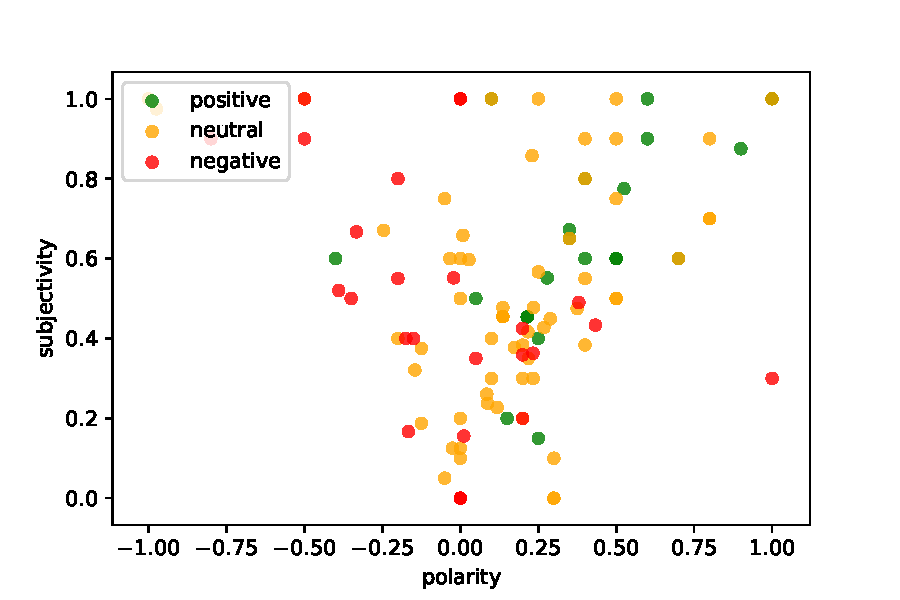
\includegraphics[width=\textwidth]{../figures/textblob.pdf}
    \end{subfigure}%
    \begin{subfigure}{.5\textwidth}
        \centering
        \caption{Google Cloud natural language API}
        \label{fig:gcloud}
        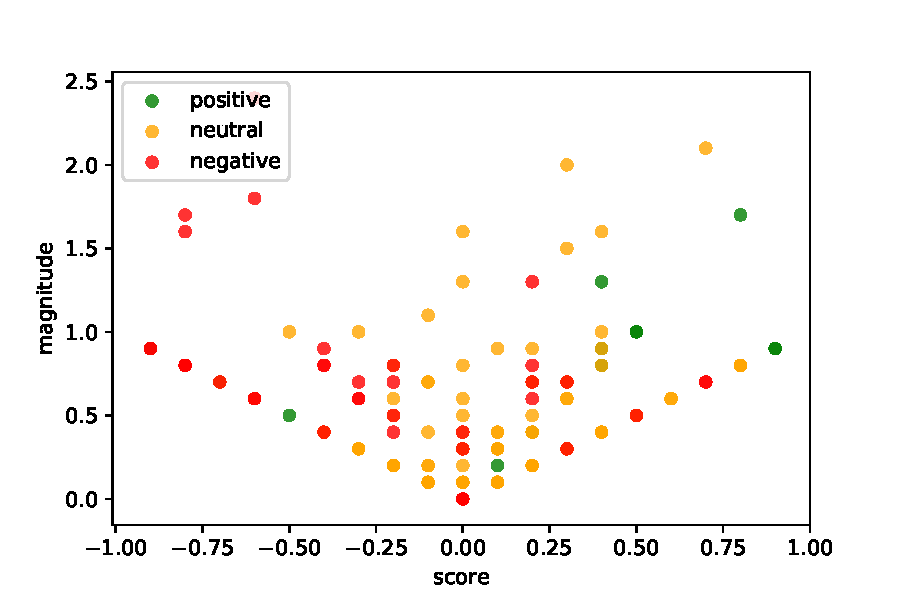
\includegraphics[width=\textwidth]{../figures/gcloud.pdf}
    \end{subfigure}
\end{figure}

As for the VADER-classifier in~\cref{subsec:vader}, these values are mapped to the labels from the dataset by
choosing an optimal threshold for which a status will be classified as neutral.
Statuses labeled as irrelevant were, again, discarded.
The optimal magnitude-threshold was found at a magnitude of 0.9, giving an accuracy of 49\%,
which is just marginally better than guessing neutral, with 47\% of statuses being labeled neutral.

\begin{equation}
    class(x) =
    \begin{cases}
        neutral & \text{for } |compound\_sentiment(x)| < 0.9 \\
        positive & \text{for } compound\_sentiment(x) \geq 0.9 \\
        negative & \text{for } compound\_sentiment(x) \leq -0.9 \\
    \end{cases}
\end{equation}

\section{Comparison and Conclusion}
\label{sec:comparison}

When comparing the results of the different methods presented, it is surprising to see the simplest,
a multinomial naive Bayes, turned out to be the most accurate.
The summarized accuracy results can be seen in~\cref{tab:sa_results}.


This indicates that short text statuses on micro-blogs like Twitter present a special challenge to sentiment analysis
that cannot be solved with current approaches.
Additions to existing algorithms, like marking negated words, that showed improved results with regular texts,
showed no improvement to the multinomial naive Bayes classifier when working with Twitter statuses.
Furthermore, even methods specifically designed for this special challenge, like VADER,
were outperformed by a multinomial naive Bayes classifier.

However, the results of these tests need to be handled carefully.
As explained in~\cref{sec:theSandersDataset},
and also indicated by the performance discrepancies between different dictionaries in~\cref{subsec:naivebayes},
the dataset used is highly topical.

The sample stream dataset introduced in~\cref{sec:streamingSampleDataset} was then classified using the multinomial naive bayes classifier from~\cref{subsec:naivebayes}.
When comparing the sentiment distribution of this dataset, seen in~\cref{fig:sample_sentiment},
to that of the Sanders dataset, seen in~\cref{fig:sanders_sentiment},
one can see that it seems to be more opinionated,
containing fewer statuses labeled as "irrelevant" in favor of positive and negative tweets.

This indicates that the dataset is not only highly topical, but also not perfectly representative in terms of sentiment.
Still, the multinomial naive Bayes classifier was saved and will be used in the upcoming chapters.

\begin{table}[t]
    \begin{minipage}[t]{.5\textwidth }
        \captionof{table}{Sentiment classification accuracy comparison}
        \label{tab:sa_results}
        \centering
        \resizebox{\textwidth}{!}{%
        \begin{tabular}{lll} %
            \toprule
            Method
            & Statuses used
            & Accuracy
            \\\midrule
            & \textit{all} & 75\%
            \\\cmidrule{2-3}
            Naive Bayes & positive, negative, neutral & 74\%
            \\\cmidrule{2-3}
            & positive, negative & 72\%
            \\\midrule
            NLTK Sentiment Analyzer & \textit{all} & 75\%
            \\\midrule
            VADER & positive, negative, neutral & 68\%
            \\\midrule
            TextBlob & positive, negative & 64\%
            \\\midrule
            Google Cloud Platform & positive, negative, neutral & 49\%
            \\\bottomrule
        \end{tabular}}
    \end{minipage}%
    \hfill
    \begin{minipage}[t]{.46\textwidth}
        \centering
        \captionof{figure}{Sample stream dataset label distribution}
        \label{fig:sample_sentiment}
        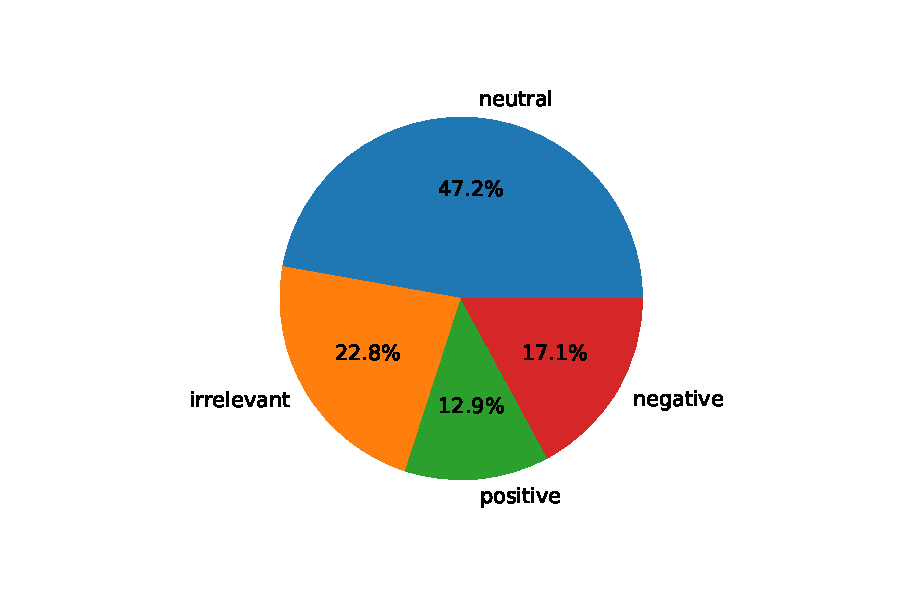
\includegraphics[width=\textwidth]{../figures/sample_sentiment.pdf}
    \end{minipage}
\end{table}